\documentclass[12pt,a4paper]{article}
\usepackage{amsmath, bm, empheq, geometry, graphicx, hyperref, physics, siunitx}
\usepackage[extrafootnotefeatures]{xepersian}
\settextfont{XB Zar}
\title{حل عددی معادلات ماکسول با روش تفاضل محدود حوزه زمان\LTRfootnote{Finite-Difference Time-Domain}}
\author{صالح شاملو احمدی\\دانشگاه صنعتی شریف، دانشکده فیزیک}
\date{18 تیر 1400}

\hypersetup{colorlinks=true, citecolor=cyan, urlcolor=blue}

\renewcommand\d[1]{\mathop{d#1}}
\newcommand{\disder}[2]{\frac{\Delta{#1}}{\Delta{#2}}}
\newcommand{\qfrac}[2]{\left(\frac{#1}{#2}\right)}
\newcommand{\fsqrt}[2]{\sqrt{\frac{#1}{#2}}}
\newcommand{\ddfrac}[2]{{\displaystyle\frac{\displaystyle #1}{\displaystyle #2}}}
\newcommand{\pdvc}[3]{\qfrac{\partial #1}{\partial #2}_{#3}}
\newcommand{\dbar}{{d\mkern-7mu\mathchar'26\mkern-2mu}}
\newcommand*{\defeq}{\mathrel{\vcenter{\baselineskip0.5ex \lineskiplimit0pt
						\hbox{\scriptsize.}\hbox{\scriptsize.}}}
						=}

\begin{document}
	\maketitle
	\begin{abstract}
		روش تفاضل محدود حوزه زمان (به اختصار \lr{FDTD}) روشی نسبتاً ساده برای حل عددی معادلات ماکسول است.
		این روش با گسسته‌سازی میدان‌ها و فضازمان، مقدار میدان‌ها را در هر لحظه از زمان با کمک معادلات ماکسول به صورت موضعی به ‌روزرسانی می‌کند.
		در این مقاله روش پیاده‌سازی و کاربرد FDTD را بررسی می‌کنیم.
	\end{abstract}
	\section{معادلات ماکسول}
	معادلات ماکسول عبارت‌اند از
	\begin{empheq}[left=\empheqlbrace]{align}
		\div{\vb{D}}&=\rho &(\text{قانون گاوس}), \\
		\div{\vb{B}}&=0 &(\text{قانون مغناطیسی گاوس}), \\
		\curl{\vb{E}}&=-\pdv{\vb{B}}{t} &(\text{قانون فارادی}), \\
		\curl{\vb{H}}&=\vb{J}+\pdv{\vb{D}}{t} &(\text{قانون آمپر-ماکسول}).
	\end{empheq}
	در این شکل از معادلات ماکسول، $\rho$ و $\vb{J}$ چگالی بار آزاد و چگالی جریان آزاد را نشان می‌دهند.
	پس در محیط‌های خطی در نقاطی که منبع (بار و جریان آزاد) وجود ندارد
	\begin{empheq}[left=\empheqlbrace]{align}
		\div{\vb{E}}&=0, \\
		\div{\vb{H}}&=0, \\
		\curl{\vb{E}}&=-\mu\,\pdv{\vb{H}}{t}, \\
		\curl{\vb{H}}&=\epsilon\,\pdv{\vb{E}}{t}.
	\end{empheq}
	در مختصات دکارتی و به صورت گسسته
	\begin{empheq}[left=\empheqlbrace]{align}
		\epsilon\,\disder{E_x}{t} &= \disder{H_z}{y} - \disder{H_y}{z}, \\
		\epsilon\,\disder{E_y}{t} &= \disder{H_x}{z} - \disder{H_z}{x}, \\
		\epsilon\,\disder{E_z}{t} &= \disder{H_y}{x} - \disder{H_x}{y},
	\end{empheq}
	\begin{empheq}[left=\empheqlbrace]{align}
		\mu\,\disder{H_x}{t} &= \disder{E_y}{z} - \disder{E_z}{y}, \\
		\mu\,\disder{H_y}{t} &= \disder{E_z}{x} - \disder{E_x}{z}, \\
		\mu\,\disder{H_z}{t} &= \disder{E_x}{y} - \disder{E_y}{x}.
	\end{empheq}
	مرسوم است که در الکترومغناطیس محاسباتی به جای میدان $B$، میدان $H$ محاسبه شود.
	این کمیت در کار تجربی (آزمایشگاهی و صنعتی) سودمندتر است.
	\section{روش FDTD}
	روش تفاضل محدود حوزه زمان (FDTD) اولین بار توسط کِین شی-گونگ یی\LTRfootnote{Kane Shee-Gong Yee} در سال 1966 ارائه شد.
	دلیل این نامگذاری برای روش این است که میدان‌ها با اختلاف میدان‌های نقاط مجاور به صورت موضعی بدست می‌آیند و همچنین حل
	روی دامنه زمانی انجام می‌شود و تحول زمانی سیستم را نشان می‌دهد.
	\subsection{گسسته‌سازی}
	\begin{figure}
		\centering
		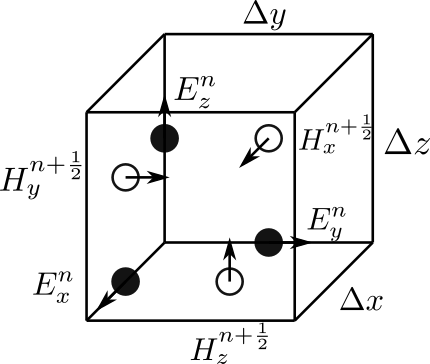
\includegraphics[width=0.6\linewidth]{yee_cell}
		\caption{یک سلول در شبکه یی}
		\label{yee cell}
	\end{figure}
	\begin{figure}
		\centering
		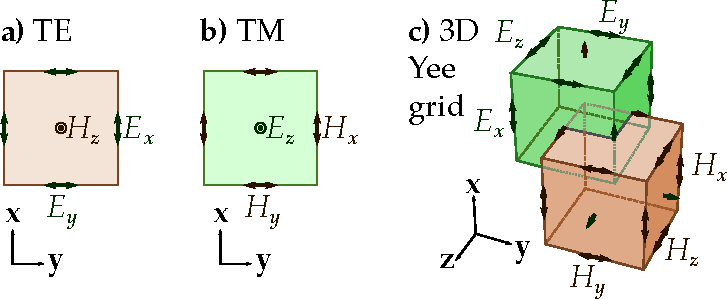
\includegraphics[width=0.6\linewidth]{yee_grid}
		\caption{شکل شبکه یی}
		\label{yee grid}
	\end{figure}
	برای دقت بالاتر محاسبات، گسسته‌سازی مطابق شکل به صورت یک در میان برای میدان‌ها انجام می‌شود.
	با تقسیم فضا به تعدادی مکعب، میدان الکتریکی را وسط اضلاع و میدان مغناطیسی را وسط وجوه سلول‌های مکعبی فضا حساب می‌کنیم.
	در شکل‌های \ref{yee cell} و \ref{yee grid} می‌توانید شکل شبکه ایجاد شده در فضا را مشاهده کنید.
	این روش گسسته‌سازی، \emph{شبکه یی}\LTRfootnote{Yee Lattice/Yee Grid} یا \emph{نگاشت یی}\LTRfootnote{Yee's Scheme} نامیده می‌شود.
	با این روند با استفاده از خصوصیات هر سلول مکعبی از فضا، میدان‌های مربوط به هر سلول را محاسبه می‌کنیم.
	
	اگر مختصات گسسته نقاط (شماره آنها بین کل نقاط) را با اعداد $(l, m, n)$،
	فاصله زمانی لحظات شبیه‌سازی را با $\Delta{t}$ و فاصله نقاط شبکه (طول ضلع سلول مکعبی شبکه) را با $\delta$ نشان دهیم،
	با گسسته سازی معادلات ماکسول (در محیط خطی در جایی که بار و جریان آزاد نداریم)
	\begin{align}
		\begin{split}
			E_x^{l,m,n}(t + \Delta{t}) &= E_x^{l,m,n}(t) \\
			&+ \frac{\Delta{t}}{\epsilon}\qty(\frac{H_z^{l,m+1/2,n}-H_z^{l,m-1/2,n}}{\delta_y}-\frac{H_y^{l,m,n+1/2}-H_y^{l,m,n-1/2}}{\delta_z}),
		\end{split}\\
		\begin{split}
			E_y^{l,m,n}(t + \Delta{t}) &= E_y^{l,m,n}(t) \\
			&+ \frac{\Delta{t}}{\epsilon}\qty(\frac{H_x^{l,m,n+1/2}-H_x^{l,m,n-1/2}}{\delta_z}-\frac{H_z^{l+1/2,m,n}-H_z^{l-1/2,m,n}}{\delta_x}),
		\end{split}\\
		\begin{split}
			E_z^{l,m,n}(t + \Delta{t}) &= E_z^{l,m,n}(t) \\
			&+ \frac{\Delta{t}}{\epsilon}\qty(\frac{H_y^{l+1/2,m,n}-H_y^{l-1/2,m,n}}{\delta_x}-\frac{H_x^{l,m+1/2,n}-H_x^{l,m-1/2,n}}{\delta_y}),
		\end{split}
	\end{align}
	\begin{align}
		\begin{split}
			H_x^{l,m,n}(t + \Delta{t}) &= H_x^{l,m,n}(t) \\
			&+ \frac{\Delta{t}}{\mu}\qty(\frac{E_y^{l,m,n+1/2}-E_y^{l,m,n-1/2}}{\delta_z}-\frac{E_z^{l,m+1/2,n}-E_z^{l,m-1/2,n}}{\delta_y}),
		\end{split}\\
		\begin{split}
			H_y^{l,m,n}(t + \Delta{t}) &= H_y^{l,m,n}(t) \\
			&+ \frac{\Delta{t}}{\mu}\qty(\frac{E_z^{l+1/2,m,n}-E_z^{l-1/2,m,n}}{\delta_x}
			-\frac{E_x^{l,m,n+1/2}-E_x^{l,m,n-1/2}}{\delta_z}),
		\end{split}\\
		\begin{split}
			H_z^{l,m,n}(t + \Delta{t}) &= H_z^{l,m,n}(t) \\
			&+ \frac{\Delta{t}}{\mu}\qty(\frac{E_x^{l,m+1/2,n}-E_x^{l,m-1/2,n}}{\delta_y}-\frac{E_y^{l+1/2,m,n}-E_y^{l-1/2,m,n}}{\delta_x}).
		\end{split}
	\end{align}
	این معادلات را بر حسب سرعت نور در خلأ $c=\flatfrac{1}(\sqrt{\mu_0\epsilon_0})$، امپدانس خلأ $Z_0\defeq\sqrt{\mu_0/\epsilon_0}$
	ضریب گذردهی نسبی (ضریب دی‌الکتریک) $\epsilon_r\defeq\epsilon/\epsilon_0 $، ضریب پذیرفتاری نسبی $\mu_r\defeq\mu/\mu_0 $ و
	\emph{عدد کورانت}\LTRfootnote{Courant Number} $C_0\defeq c\Delta{t}/\delta$ بازنویسی می‌کنیم (فرض می‌کنیم فواصل شبکه در تمام جهات یکسان هستند):
	\begin{align}
		\begin{split}
			E_x^{l,m,n}(t + \Delta{t}) &= E_x^{l,m,n}(t) \\
			&+ \frac{C_0 Z_0}{\epsilon_r}\qty[\qty(H_z^{l,m+1/2,n}-H_z^{l,m-1/2,n})-\qty(H_y^{l,m,n+1/2}-H_y^{l,m,n-1/2})],
		\end{split} \\
		\begin{split}
			E_y^{l,m,n}(t + \Delta{t}) &= E_y^{l,m,n}(t) \\
			&+ \frac{C_0 Z_0}{\epsilon_r}\qty[\qty(H_x^{l,m,n+1/2}-H_x^{l,m,n-1/2})-\qty(H_z^{l+1/2,m,n}-H_z^{l-1/2,m,n})], 
		\end{split}\\
		\begin{split}
			E_z^{l,m,n}(t + \Delta{t}) &= E_z^{l,m,n}(t) \\
			&+ \frac{C_0 Z_0}{\epsilon_r}\qty[\qty(H_y^{l+1/2,m,n}-H_y^{l-1/2,m,n})-\qty(H_x^{l,m+1/2,n}-H_x^{l,m-1/2,n})],
		\end{split}
	\end{align}
	\begin{align}
		\begin{split}
			H_x^{l,m,n}(t + \Delta{t}) &= H_x^{l,m,n}(t) \\
			&+ \frac{C_0}{Z_0\mu_r}\qty[\qty(E_y^{l,m,n+1/2}-E_y^{l,m,n-1/2})-\frac{E_z^{l,m+1/2,n}-E_z^{l,m-1/2,n}}{\delta_y}],
		\end{split}\\
		\begin{split}
			H_y^{l,m,n}(t + \Delta{t}) &= H_y^{l,m,n}(t) \\
			&+ \frac{C_0}{Z_0\mu_r}\qty[\qty(E_z^{l+1/2,m,n}-E_z^{l-1/2,m,n})-\qty(E_x^{l,m,n+1/2}-E_x^{l,m,n-1/2})],
		\end{split}\\
		\begin{split}
			H_z^{l,m,n}(t + \Delta{t}) &= H_z^{l,m,n}(t) \\
			&+ \frac{C_0}{Z_0\mu_r}\qty[\qty(E_x^{l,m+1/2,n}-E_x^{l,m-1/2,n})-\qty(E_y^{l+1/2,m,n}-E_y^{l-1/2,m,n})].
		\end{split}
	\end{align}
	با استفاده مکرر از این معادلات در هر گام زمانی، می‌توانیم تحول میدان‌ها را شبیه‌سازی کنیم و وضعیت سیستم را در زمان‌های مختلف پیدا کنیم.
	\subsection{پایداری}
	طبق شرط همگرایی کورانت-فردریشز-لوی\LTRfootnote{Courant–Friedrichs–Lewy Convergence Condition}، شرط پایداری الگوریتم FDTD این است که
	عدد کورانت کوچک‌تر مساوی عکس رادیکال بُعد فضا باشد. یعنی به عنوان مثال در سه بعد $C_0\le1/\sqrt{3}$.
	این یک شرط محاسباتی مربوط به حل عددی معادلات دیفرانسیل است، اما به صورت فیزیکی نیز می‌توانیم آن را تعبیر کنیم:
	اطلاعات با سرعت نور انتقال پیدا می‌کند، پس در هر مرحله میدان‌های سلول‌هایی که فاصله آنها از $c\Delta{t}$ کمتر باشد باید توسط یک نقطه به‌روزرسانی شوند؛
	اگر عدد کورانت از مقدار حداکثری که برایش تعریف کردیم بزرگ‌تر باشد، باید علاوه بر سلول‌های همسایه، سلول‌های دورتری نیز به‌روزرسانی شوند؛
	اما در روش FDTD فقط سلول‌های همسایه در هر گام زمانی به‌روزرسانی می‌شوند، پس در این حالت الگوریتم FDTD به مشکل می‌خورد.
	
	دقت کنید که اگر عدد کورانت کوچک‌تر از مقدار حداکثر خود باشد، مقدار به‌روزرسانی شده برای سلول همسایه تقریبی از مقدار میدان در فضای بین
	خود سلول و همسایه‌اش خواهد بود، چراکه نور در این حالت در یک گام فرصت ندارد فاصله دو سلول را طی کند.
	بنابراین هرچقدر عدد کورانت به مقدار حداکثر خود نزدیک‌تر باشد، دقت جواب بالاتر خواهد بود.
	\subsection{منبع میدان}
	تا اینجا معادلات را بدون بار و جریان آزاد در نظر گرفتیم. در حالت کلی‌تر، چگالی بار و جریان منابعی برای تولید میدان هستند.
	\subsection{جریان}
	اگر در یک نقطه از فضا چگالی جریان $\vb{J}$ داشته باشیم
	\begin{equation}
		\curl{\vb{H}}=\vb{J}+\epsilon\pdv{\vb{E}}{t},
	\end{equation}
	یا به شکل گسسته
	\begin{equation}
		\Delta{\vb{E}}=-\frac{\Delta{t}}{\epsilon}\,\vb{J}+\Delta{t}\curl{\vb{H}}.
	\end{equation}
	بدین ترتیب می‌توانیم تغییرات میدان را به دو بخش تقسیم کنیم:
	\begin{equation}
		\Delta{\vb{E}}=\Delta{\vb{E}}_s + \Delta{\vb{E}}_H
	\end{equation}
	جمله $\Delta{\vb{E}}_H$ مربوط به اثر میدان مغناطیسی است که در بخش قبل گسسته‌سازی کردیم.
	جمله $\Delta{\vb{E}}_s$ مربوط به اثر چگالی جریان است که در نقاطی که جریان داریم به مقدار قبلی اضافه می‌شود.
	بنابراین جمله مربوط به چگالی جریان مانند یک منبع برای میدان الکتریکی عمل می‌کند.
	
	شاید کمی عجیب به نظر بیاید که چگالی جریان به جای میدان مغناطیسی منبع میدان الکتریکی باشد، چراکه معادلات ماکسول تصویر دیگری ارائه می‌دهند.
	نکته قابل توجه این است که در سیستم‌های واقعی (که آنها را با روش‌های عددی شبیه‌سازی می‌کنیم) جریان‌ها و میدان‌ها پایا نیستند
	(هرچند در طول زمان ممکن است به یک حالت پایدار برسند)، بنابراین در هر نقطه از فضا میدان الکتریکی و مغناطیسی داریم متغیر داریم که روی هم تأثیر می‌گذارند.
	بنابراین یک منبع برای هر کدام از میدان‌های مغناطیسی و الکتریکی، باعث تولید میدان دیگر هم می‌شود.
	\subsection{بار}
	طبق قانون گاوس در محیط‌های خطی
	\begin{equation}
		\div{\vb{E}} = \frac{\rho}{\epsilon}.
	\end{equation}
	مشابه چگالی جریان، بار نیز مثل یک منبع برای میدان الکتریکی عمل می‌کند، با این تفاوت که اثر آن به طور ثابت به میدان اضافه می‌شود؛
	یعنی با گذر زمان اثر آن روی میدان افزایش پیدا نمی‌کند و تنها در فضا پخش می‌شود.
	
	با توجه به نتایج بدست آمده، در کلی‌ترین حالت برای در نظر گرفتن اثر بار و جریان می‌توانیم در معادلات یک جمله منبع $\vb{E}_s$ اضافه کنیم.
	\section{شرایط مرزی}
	اگر در مرزهای فضای شبیه‌سازی تغییری اعمال نکنیم و میدان را در آنجا برابر صفر قرار دهیم، این مرزها مانند آینه عمل می‌کنند
	و میدان‌ها را بازتاب می‌کنند. در شبیه‌سازی سیستم‌ها به طور معمول سیستم‌ها را داخل فضای آزاد بررسی می‌کنیم؛
	یعنی محیط به نسبت سیستم مورد بررسی خیلی بزرگ‌تر است و انگار داریم یک بخش کوچک از فضا را بررسی می‌کنیم.
	بنابراین مرزهای بازتاب‌کننده برای بیشتر شبیه‌سازی‌ها مناسب نیستند.
	
	برای شبیه‌سازی یک سیستم داخل فضای آزاد باید از \emph{شرایط مرزی جذب کننده}\LTRfootnote{Absorbing Boundary Conditions} استفاده کنیم؛
	دیواره‌ها با این نوع شرایط مرزی با تقلید میدان‌ها در نقاط همسایه خود می‌توانند میدان‌ها را جذب کنند و از بازتاب شدن آنها جلوگیری کنند.
	انگار که سیگنال از دیواره‌ها عبور کرده و وارد فضای آزاد شده.
	
	پیاده‌سازی شرایط مرزی جذب‌کننده فقط در یک بُعد به طور دقیق ممکن است و در ابعاد بالاتر به طور تقریبی امکان پذیر است.
	\section{نقاط قوت FDTD}
	\begin{enumerate}
		\item این روش نسبت به بقیه روش‌های حل معادلات ماکسول ساده‌تر است و پیاده‌سازی آن نسبتاً آسان است
		\item چون جواب‌ها برحسب زمان هستند (برخلاف بعضی روش‌ها که جوابشان بر حسب فرکانس است)، می‌توان دامنه وسیعی از فرکانس‌ها را در یک شبیه‌سازی بررسی کرد
		\item تعمیم این روش برای جزئیات مختلف برای فضا و محیط‌های غیر خطی ساده است 
	\end{enumerate}
	\section{نقاط ضعف FDTD}
	\begin{enumerate}
		\item به دلیل روش گسسته‌سازی به کار رفته، در مواردی که میدان تغییر ناگهانی دارد در جواب اختلالاتی به وجود می‌آید (پدیده گیبس)
		\item فاصله نقاط شبکه در این روش باید هم از کوچک‌ترین جزئیات سیستم و هم اس کوچک‌ترین طول موج کوتاه‌تر باشد.
		در بعضی موارد مثل سیم‌های نازک این موضوع باعث می‌شود محاسبات بسیار سنگین شود.
	\end{enumerate}
	\section{مثال‌ها}
	\subsection{موج سینوسی}
	\begin{center}
		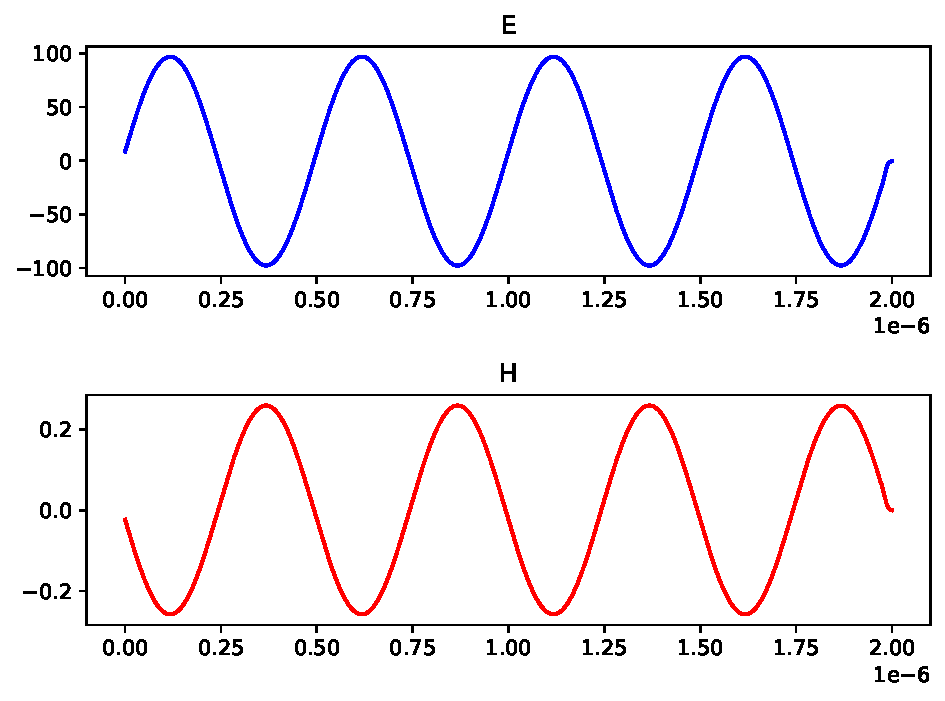
\includegraphics{sin}
	\end{center}
	\subsection{عبور موج سینوسی از یک برش ماده خطی}
	در شکل زیر بین $\SI{1.0}{\micro\meter}$ و $\SI{1.2}{\micro\meter} $ یک برش از ماده‌ای با ضریب شکست $\sqrt{3}$ قرار دارد.
	\begin{center}
		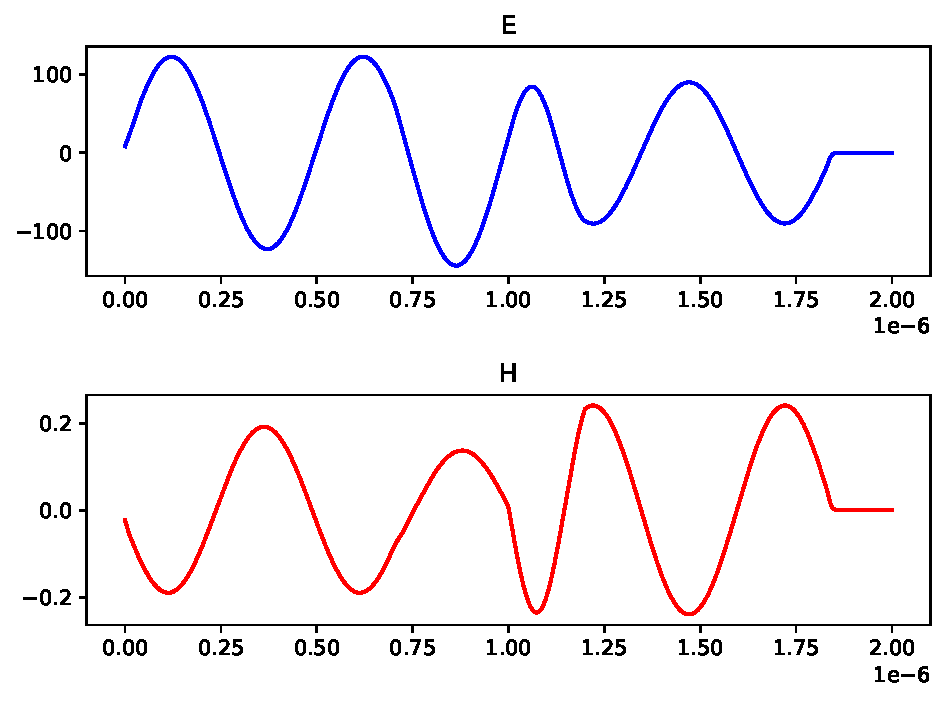
\includegraphics{slab}
	\end{center}
	\subsection{موج مربعی}
	\begin{center}
		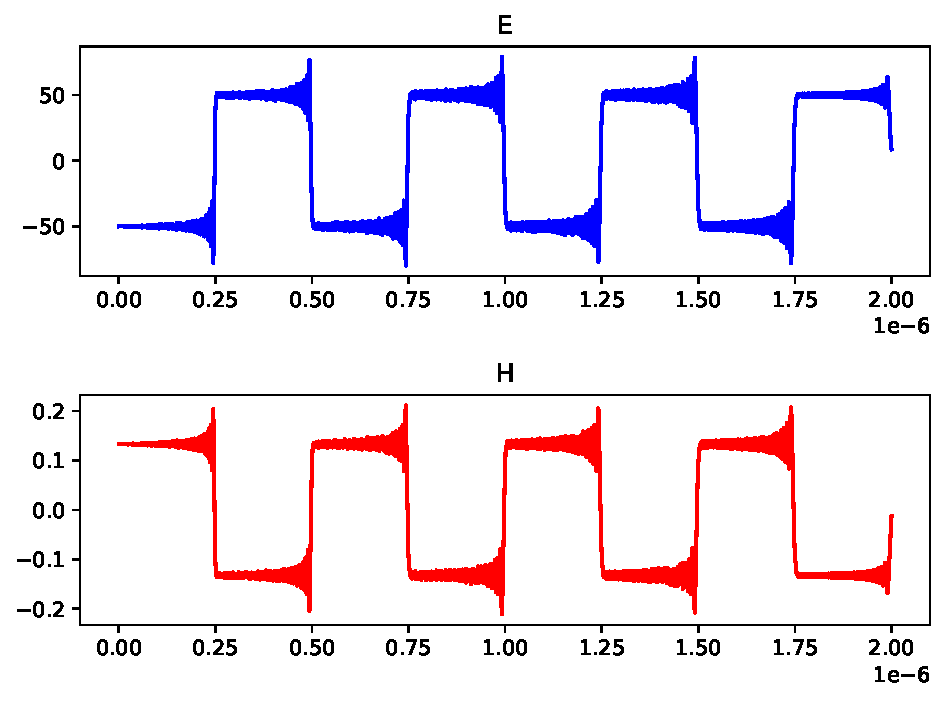
\includegraphics{rect}
	\end{center}
	\subsection{منبع خطی در یک بعد}
	\begin{center}
		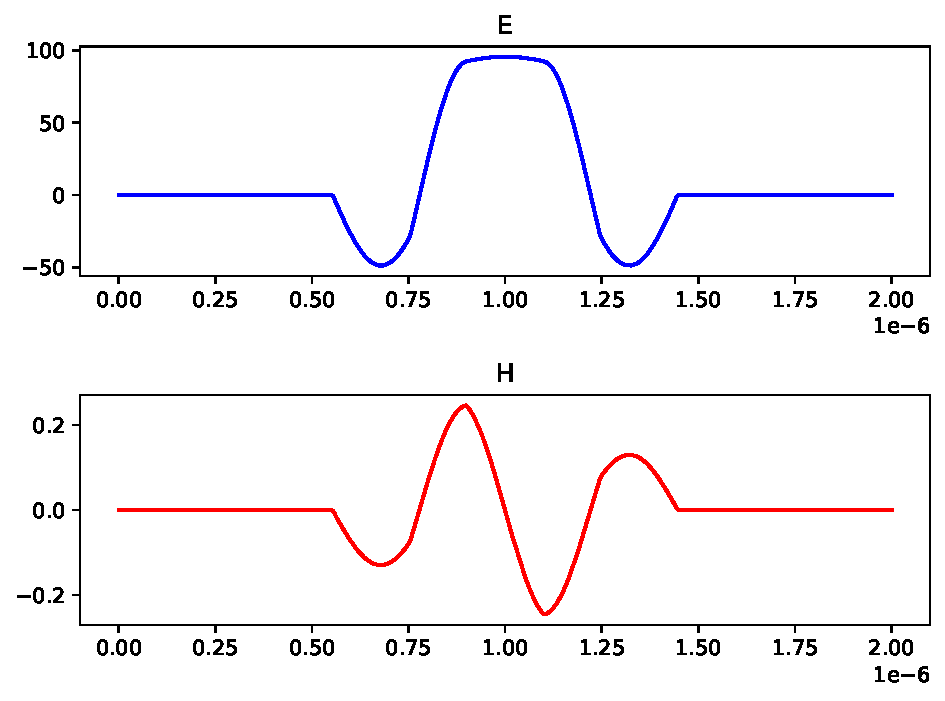
\includegraphics{line1d2}
	\end{center}
	\begin{center}
		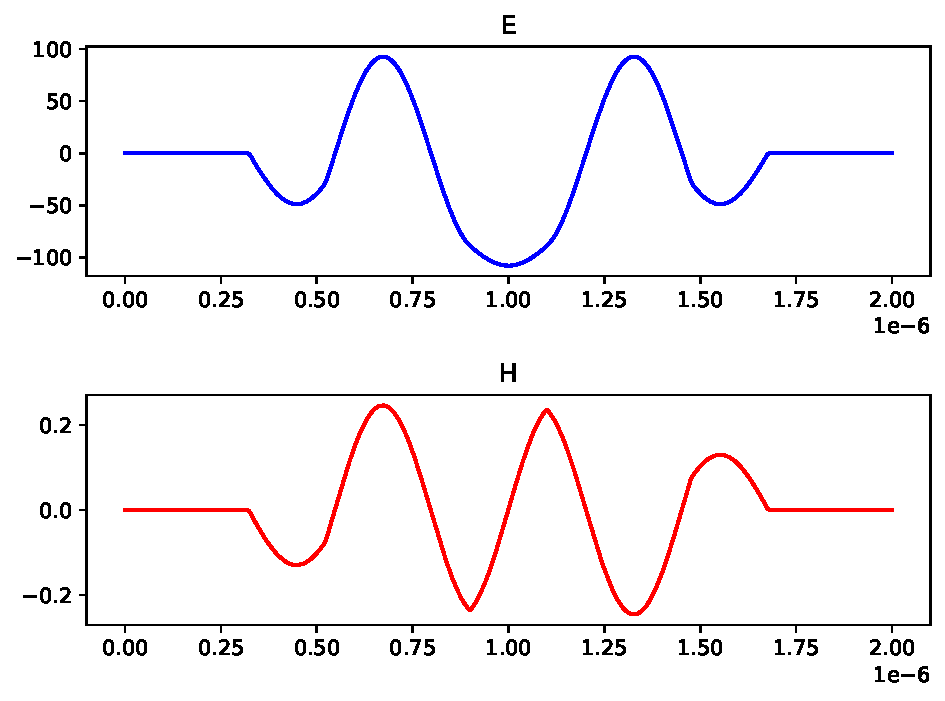
\includegraphics{line1d}
	\end{center}
	\subsection{منبع خطی در دو بعد}
	\begin{center}
		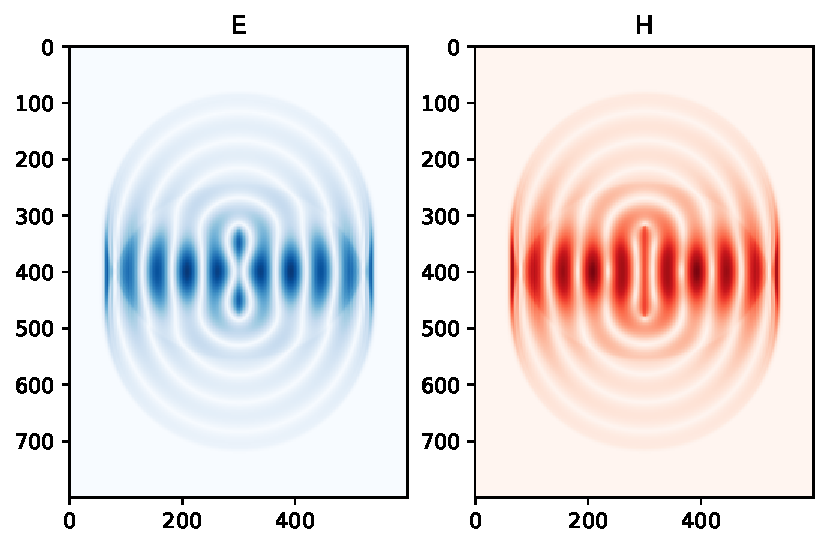
\includegraphics{line2d}
	\end{center}
	\subsection{دوقطبی}
	\begin{center}
		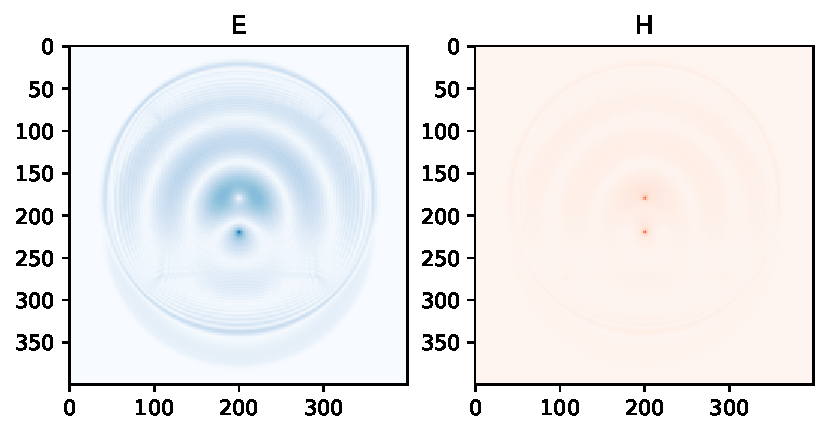
\includegraphics{dipole}
	\end{center}
	\begin{center}
		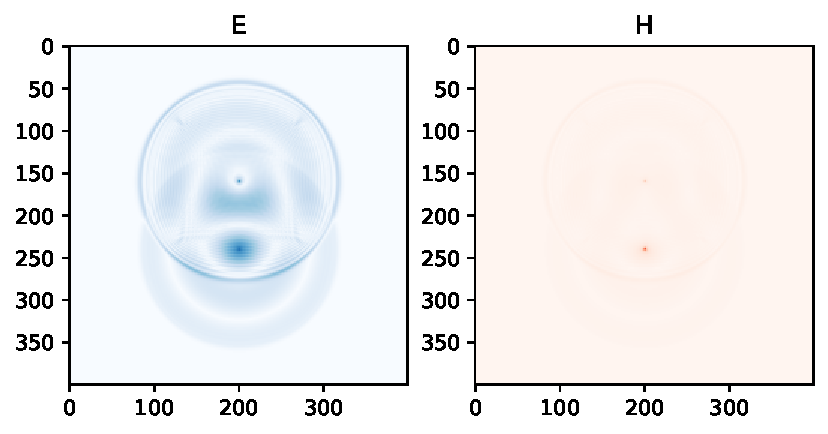
\includegraphics{dipole2}
	\end{center}
	\begin{center}
		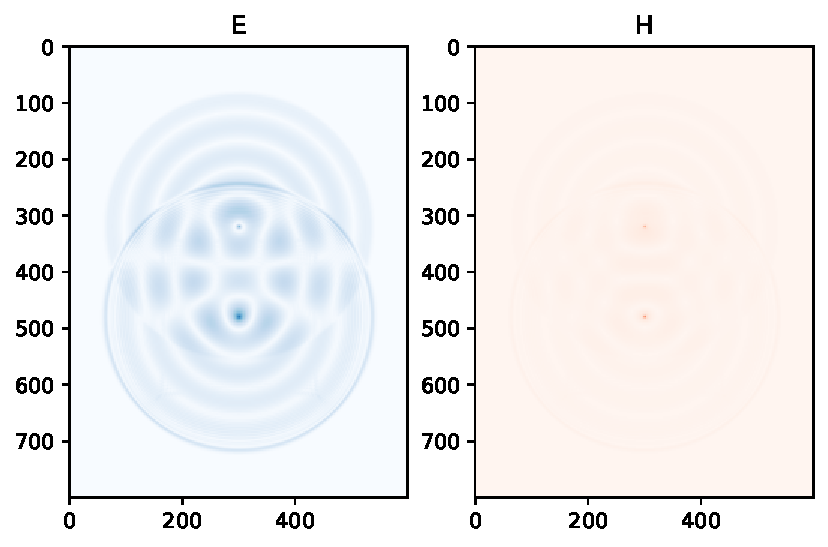
\includegraphics{dipole3}
	\end{center}
\end{document}
